\chapter{A dissolução dos sólidos iônicos e moleculares}\label{ch:g11:dissolution}

Uma pitada de sal mexida na água some em segundos; a mesma pitada mexida
no óleo de cozinha fica no fundo do copo, sem mudar, por quanto tempo
alguém quiser olhar. Uma frigideira engordurada enxaguada na torneira
continua engordurada; uma gota de detergente, e a gordura se solta. O
que decide se uma substância \omterm{def:g2:mixing-and-dissolving:dissolve}{se dissolve} num líquido? A resposta está
nas \omterm{def:g11:polarity-and-cohesion:polar-bond}{cargas parciais} e nas forças entre partículas do capítulo anterior.

\begin{recall}
A \omterm{def:g6:solutions-and-solubility:solubility}{solubilidade}; os líquidos \omterm{def:g6:solutions-and-solubility:miscible}{miscíveis} e \omterm{def:g6:solutions-and-solubility:miscible}{imiscíveis}
(\cref{ch:g6:solutions-and-solubility}). Um \omterm{def:g9:ions:ionic-compound}{composto iônico} é formado
por \omterm{def:g9:ions:ion}{cátions} e \omterm{def:g9:ions:ion}{ânions} em proporções que o tornam neutro
(\cref{ch:g9:ions}). As \omterm{def:g11:polarity-and-cohesion:polar-molecule}{moléculas polares} e apolares, as \omterm{def:g11:polarity-and-cohesion:hydrogen-bond}{ligações de
hidrogênio}, as \omterm{def:g11:polarity-and-cohesion:van-der-waals}{interações de van der Waals}
(\cref{ch:g11:polarity-and-cohesion}). A \omterm{def:g10:chemical-species:extraction}{extração líquido--líquido}
(\cref{ch:g10:chemical-species}). A \omterm{def:g10:concentration-and-dilution:molar-concentration}{concentração molar}
(\cref{ch:g10:concentration-and-dilution}).
\end{recall}

\section{A dissolução de um sólido iônico}

Num cristal de cloreto de sódio, cada \omterm{def:g9:ions:ion}{íon} sódio \ce{Na+} está cercado por
\omterm{def:g9:ions:ion}{íons} cloreto \ce{Cl-} e cada \omterm{def:g9:ions:ion}{íon} cloreto por \omterm{def:g9:ions:ion}{íons} sódio, todos mantidos
pela atração entre cargas opostas. As \omterm{def:g7:atoms-and-molecules:molecule}{moléculas} de água, polares, são
atraídas por essas cargas: o seu lado do oxigênio ($\delta^-$) se volta
para os \omterm{def:g9:ions:ion}{cátions}, o seu lado dos hidrogênios ($\delta^+$) para os \omterm{def:g9:ions:ion}{ânions}.

\begin{definition}[Dissociação]\label{def:g11:dissolution:dissociation}
A \emph{dissociação}\index{dissociacao@dissociação} de um sólido iônico num \omterm{def:g6:solutions-and-solubility:solute}{solvente}
é a separação dos seus \omterm{def:g9:ions:ion}{íons} uns dos outros: eles deixam o cristal e se
afastam na solução.
\end{definition}

\begin{definition}[Solvatação, hidratação]\label{def:g11:dissolution:solvation}
A \emph{solvatação}\index{solvatacao@solvatação} de uma partícula dissolvida é o seu
envolvimento por \omterm{def:g7:atoms-and-molecules:molecule}{moléculas} de \omterm{def:g6:solutions-and-solubility:solute}{solvente}, presas a ela por atrações; na
água, ela se chama \emph{hidratação}\index{hidratacao@hidratação}. O símbolo (aq)
depois de uma fórmula quer dizer ``hidratado''.
\end{definition}

\begin{proposition}[As três etapas da dissolução]\label{prop:g11:dissolution:stages}
Um sólido iônico \omterm{def:g2:mixing-and-dissolving:dissolve}{se dissolve} na água em três etapas que acontecem
juntas: os \omterm{def:g9:ions:ion}{íons} são arrancados do cristal (\omterm{def:g11:dissolution:dissociation}{dissociação}), envolvidos por
\omterm{def:g7:atoms-and-molecules:molecule}{moléculas} de água (\omterm{def:g11:dissolution:solvation}{hidratação}) e espalhados por toda a solução
(dispersão). Para o cloreto de sódio,
\[
  \ce{NaCl(s) -> Na+(aq) + Cl-(aq)} .
\]
\end{proposition}

\begin{proof}
Admitido: as atrações entre os \omterm{def:g9:ions:ion}{íons} e as \omterm{def:g11:polarity-and-cohesion:polar-molecule}{moléculas polares} de água,
somadas, são fortes o bastante para substituir as atrações entre os \omterm{def:g9:ions:ion}{íons}
do cristal.
\end{proof}

\begin{omfigure}
\begin{tikzpicture}[font=\small]
  % the crystal edge: alternating ions
  \foreach \i in {0,1,2,3,4} \foreach \j in {0,1,2,3} {
    \pgfmathtruncatemacro\k{mod(\i+\j,2)}
    \ifnum\k=0
      \node[om atom, ball color=green!60!black, minimum size=6.4mm] at (0.8*\i,0.8*\j) {};
    \else
      \node[om atom, ball color=violet!70, minimum size=4.0mm] at (0.8*\i,0.8*\j) {};
    \fi
  }
  % a hydrated Na+ that has left: O towards the ion
  \begin{scope}[shift={(5.6,1.8)}]
    \node[om atom, ball color=violet!70, minimum size=4.0mm] (na) at (0,0) {};
    \node[font=\footnotesize] at (0,0) {};
    \foreach \a in {0,90,180,270} {
      \node[aO, minimum size=4.6mm] (o\a) at (\a:0.62) {};
      \node[aH, minimum size=3.2mm] (ha\a) at ($(\a:0.62)+(\a+52:0.42)$) {};
      \node[aH, minimum size=3.2mm] (hb\a) at ($(\a:0.62)+(\a-52:0.42)$) {};
      \begin{scope}[on background layer]
        \draw[bond, line width=1.2pt] (o\a.center) -- (ha\a.center);
        \draw[bond, line width=1.2pt] (o\a.center) -- (hb\a.center);
      \end{scope}
    }
    \node[anchor=north] at (0,-1.35) {\ce{Na+(aq)}};
  \end{scope}
  % a hydrated Cl- that has left: H towards the ion
  \begin{scope}[shift={(8.6,1.4)}]
    \node[om atom, ball color=green!60!black, minimum size=6.4mm] at (0,0) {};
    \foreach \a in {45,135,225,315} {
      \node[aH, minimum size=3.2mm] (h\a) at (\a:0.62) {};
      \node[aO, minimum size=4.6mm] (o\a) at (\a:1.0) {};
      \node[aH, minimum size=3.2mm] (k\a) at ($(\a:1.0)+(\a+75:0.42)$) {};
      \begin{scope}[on background layer]
        \draw[bond, line width=1.2pt] (o\a.center) -- (h\a.center);
        \draw[bond, line width=1.2pt] (o\a.center) -- (k\a.center);
      \end{scope}
    }
    \node[anchor=north] at (0,-1.45) {\ce{Cl-(aq)}};
  \end{scope}
  \node[anchor=north, align=center] at (1.6,-0.45) {o cristal\\
    (\ce{Na+} pequeno, \ce{Cl-} grande)};
\end{tikzpicture}

{\small O cloreto de sódio se dissolvendo. Um \omterm{def:g9:ions:ion}{íon} sódio e um \omterm{def:g9:ions:ion}{íon} cloreto
deixaram o cristal; cada um está hidratado. Em volta do \omterm{def:g9:ions:ion}{cátion}, as
\omterm{def:g7:atoms-and-molecules:molecule}{moléculas} de água voltam os seus \omterm{def:g7:atoms-and-molecules:atom}{átomos} de oxigênio (vermelhos,
$\delta^-$) para dentro; em volta do \omterm{def:g9:ions:ion}{ânion}, os seus \omterm{def:g7:atoms-and-molecules:atom}{átomos} de hidrogênio
(brancos, $\delta^+$).}
\end{omfigure}

\section{As concentrações dos íons}

\begin{method}[A concentração de cada íon]\label{met:g11:dissolution:ions}
\begin{enumerate}
  \item Escreva a equação de dissolução, balanceada em \omterm{def:g7:atoms-and-molecules:atom}{átomos} e em
        carga: para o cloreto de cálcio,
        \ce{CaCl2(s) -> Ca^{2+}(aq) + 2Cl-(aq)}.
  \item Calcule a quantidade $n$ de sólido dissolvido, e a concentração
        $c = n / V$ da solução em \omterm{def:g6:solutions-and-solubility:solute}{soluto}.
  \item Cada \omterm{def:g9:ions:ion}{íon} tem a concentração $c$ multiplicada pelo seu coeficiente
        na equação: aqui $[\ce{Ca^{2+}}] = c$ e
        $[\ce{Cl-}] = 2c$.
\end{enumerate}
Os colchetes $[\ldots]$ indicam a \omterm{def:g10:concentration-and-dilution:molar-concentration}{concentração molar} de uma espécie
dissolvida.
\end{method}

\begin{example}[O cloreto de cálcio]\label{ex:g11:dissolution:cacl2}
% ledger: aw:Ca, aw:Cl
\qty{5.55}{g} de cloreto de cálcio ($M = \qty{111.1}{g/mol}$) dissolvidos
para fazer \qty{500.0}{mL} de solução: $n = \qty{0.0500}{mol}$,
$c = \qty{0.100}{mol/L}$, logo $[\ce{Ca^{2+}}] = \qty{0.100}{mol/L}$ e
$[\ce{Cl-}] = \qty{0.200}{mol/L}$. A solução é neutra: $2 \times
0.100$ de carga positiva por litro para $1 \times 0.200$ de negativa.
\end{example}

\section{Polaridade e solubilidade}

\begin{proposition}[Semelhante dissolve semelhante]\label{prop:g11:dissolution:like}
Um \omterm{def:g6:solutions-and-solubility:solute}{solvente} polar, como a água, dissolve os sólidos iônicos e as
espécies polares, sobretudo as capazes de formar \omterm{def:g11:polarity-and-cohesion:hydrogen-bond}{ligações de hidrogênio}
com ele; um \omterm{def:g6:solutions-and-solubility:solute}{solvente} apolar, como o ciclo-hexano ou um óleo vegetal,
dissolve as espécies apolares. Os sólidos iônicos se dissolvem muito
pouco nos \omterm{def:g6:solutions-and-solubility:solute}{solventes} apolares, e as espécies apolares muito pouco na
água.
\end{proposition}

\begin{proof}
Admitido: um \omterm{def:g6:solutions-and-solubility:solute}{soluto} \omterm{def:g2:mixing-and-dissolving:dissolve}{se dissolve} bem quando as atrações que ele pode
formar com o \omterm{def:g6:solutions-and-solubility:solute}{solvente} são pelo menos tão fortes quanto as que ele rompe,
entre as suas próprias partículas e entre as \omterm{def:g7:atoms-and-molecules:molecule}{moléculas} do \omterm{def:g6:solutions-and-solubility:solute}{solvente}.
\end{proof}

\begin{example}[Três casos]\label{ex:g11:dissolution:cases}
% ledger: sol:I2-water, sol:I2-heptane
O etanol se mistura com a água em todas as proporções: o seu grupo
\ce{O-H} forma \omterm{def:g11:polarity-and-cohesion:hydrogen-bond}{ligações de hidrogênio} com a água. O sal \omterm{def:g2:mixing-and-dissolving:dissolve}{se dissolve} na
água, mas não no óleo. O iodo, \ce{I2}, uma \omterm{def:g11:polarity-and-cohesion:polar-molecule}{molécula apolar}, \omterm{def:g2:mixing-and-dissolving:dissolve}{se dissolve}
mal na água (cerca de \qty{0.3}{g/L}, uma solução marrom), mas bem nos
\omterm{def:g6:solutions-and-solubility:solute}{solventes} apolares (\qty{17}{g} por quilograma de heptano, uma solução
violeta).
\end{example}

\section{A extração líquido--líquido, explicada}

Uma \omterm{def:g10:chemical-species:extraction}{extração líquido--líquido} leva uma espécie de um \omterm{def:g6:solutions-and-solubility:solute}{solvente} para
outro, \omterm{def:g6:solutions-and-solubility:miscible}{imiscível} com o primeiro, no qual ela é mais solúvel. A regra
``semelhante dissolve semelhante'' diz que \omterm{def:g6:solutions-and-solubility:solute}{solvente} escolher.

\begin{inthelab}[Extrair o iodo]
\qty{20}{mL} de uma \omterm{def:g6:solutions-and-solubility:solute}{solução aquosa} marrom de iodo são despejados num
funil de separação com \qty{10}{mL} de ciclo-hexano. O funil é tampado,
agitado, a sua pressão é aliviada pela torneira, e ele é deixado em
repouso. Formam-se duas camadas: o ciclo-hexano, menos denso, em cima. A
camada de cima agora é violeta, a de baixo quase incolor: o iodo passou
para o ciclo-hexano. A camada de baixo é escoada pela torneira, e o iodo
é recuperado no ciclo-hexano.
\end{inthelab}

\begin{omfigure}
\begin{tikzpicture}[font=\small, scale=1.15]
  \pic[transform shape] at (0,0) {sepfunnel={orange!55!brown!70}{white}};
  \node[anchor=north, align=center] at (0,-0.15) {antes da agitação};
  \draw[omProp, <-] (0.55,2.1) -- (1.4,2.5) node[right, text=black] {ciclo-hexano};
  \draw[omProp, <-] (0.45,1.35) -- (1.4,1.2) node[right, text=black,
    align=left] {iodo aquoso\\ (marrom)};
  \pic[transform shape] at (4.6,0) {sepfunnel={orange!10}{violet!60}};
  \node[anchor=north, align=center] at (4.6,-0.15) {depois da agitação\\ e do repouso};
  \draw[omProp, <-] (5.15,2.1) -- (6.0,2.5) node[right, text=black,
    align=left] {iodo no\\ ciclo-hexano (violeta)};
  \draw[omProp, <-] (5.05,1.35) -- (6.0,1.2) node[right, text=black,
    align=left] {água, quase\\ incolor};
\end{tikzpicture}

{\small \omterm{def:g10:chemical-species:extraction}{Extração} do iodo da água com ciclo-hexano. O iodo, apolar, passa
para o \omterm{def:g6:solutions-and-solubility:solute}{solvente} apolar; o ciclo-hexano, menos denso que a água, flutua
em cima.}
\end{omfigure}

\begin{safety}{\ghs[0.82cm]{GHS02}\ghs[0.82cm]{GHS07}\ghs[0.82cm]{GHS08}\ghs[0.82cm]{GHS09}}
% ledger: ghs:I2, ghs:cyclohexane
O ciclo-hexano é altamente inflamável, o seu vapor dá sonolência, ele é
nocivo para os pulmões se ingerido e muito tóxico para os organismos
aquáticos. O iodo é nocivo em contato com a pele e se inalado. Capela de
exaustão, óculos de proteção e luvas, nenhuma chama por perto; os
resíduos orgânicos são recolhidos.
\end{safety}


\section{Os sabões e as moléculas anfifílicas}

\begin{definition}[Hidrofílico, hidrofóbico]\label{def:g11:dissolution:hydrophilic}
Uma espécie ou uma parte de uma \omterm{def:g7:atoms-and-molecules:molecule}{molécula} é
\emph{hidrofílica}\index{hidrofilico@hidrofílico} se é atraída pela água (grupos
iônicos ou polares, grupos que formam \omterm{def:g11:polarity-and-cohesion:hydrogen-bond}{ligações de hidrogênio}); ela é
\emph{hidrofóbica}\index{hidrofobico@hidrofóbico} se não é (longas cadeias de \omterm{def:g7:atoms-and-molecules:atom}{átomos}
de carbono e de hidrogênio, apolares). As espécies hidrofóbicas se
dissolvem nas gorduras e nos óleos.
\end{definition}

\begin{definition}[Molécula anfifílica, micela]\label{def:g11:dissolution:amphiphilic}
Uma \omterm{def:g7:atoms-and-molecules:molecule}{molécula} ou um \omterm{def:g9:ions:ion}{íon} \emph{anfifílico}\index{anfifilico@anfifílico} tem uma cabeça
\omterm{def:g11:dissolution:hydrophilic}{hidrofílica} e uma cauda \omterm{def:g11:dissolution:hydrophilic}{hidrofóbica}. Na água, os \omterm{def:g9:ions:ion}{íons} anfifílicos se
agrupam em \emph{micelas}\index{micela}: esferas minúsculas com as
caudas dentro, fora da água, e as cabeças na superfície, em contato com
ela.
\end{definition}

\begin{example}[Um sabão]\label{ex:g11:dissolution:soap}
% ledger: aw:C, aw:H, aw:O, aw:Na
O estearato de sódio, \ce{C17H35COONa} ($M = \qty{306.0}{g/mol}$), é um
sabão típico, feito de gorduras animais ou vegetais. Na água, ele \omterm{def:g2:mixing-and-dissolving:dissolve}{se
dissolve} na forma de \omterm{def:g9:ions:ion}{íons} sódio \ce{Na+} e \omterm{def:g9:ions:ion}{íons} estearato
\ce{C17H35COO-}: uma cabeça \ce{-COO-}, iônica, \omterm{def:g11:dissolution:hydrophilic}{hidrofílica}, e uma cauda
de 17 \omterm{def:g7:atoms-and-molecules:atom}{átomos} de carbono, \omterm{def:g11:dissolution:hydrophilic}{hidrofóbica}.
\end{example}

\begin{omfigure}
\begin{tikzpicture}[font=\small]
  % the stearate ion as a zigzag of 17 carbons + COO-
  \foreach \k in {0,1,2,3,4,5,6,7,8,9,10,11,12,13,14,15,16} {
    \pgfmathsetmacro\y{mod(\k,2)==0 ? 0 : 0.3}
    \coordinate (c\k) at (0.42*\k,\y);
  }
  \draw[line width=0.9pt] (c0) \foreach \k in {1,2,3,4,5,6,7,8,9,10,11,12,13,14,15,16} { -- (c\k) };
  \coordinate (cc) at ($(c16)+(30:0.42)$);
  \begin{scope}[on background layer]
    \fill[omDef!15, rounded corners] ($(cc)+(-0.25,-0.55)$) rectangle ($(cc)+(1.05,0.9)$);
  \end{scope}
  \draw[line width=0.9pt] (c16) -- (cc);
  \draw[line width=0.9pt] (cc) -- ++(90:0.4) node[above] {O};
  \draw[line width=0.9pt] ([xshift=1.5pt]cc) -- ++(90:0.36);
  \draw[line width=0.9pt] (cc) -- ++(-30:0.42) node[right] {O$^-$};
  \draw[omProp] ($(c0)+(0,-0.15)$) -- ++(0,-0.15) -- ($(c16)+(0,-0.3)$) -- ++(0,0.15);
  \node[omProp, anchor=north] at ($(c8)+(0,-0.32)$) {cauda hidrofóbica (17 átomos de carbono)};
  \node[omDef, anchor=south] at ($(cc)+(0.35,0.9)$) {cabeça hidrofílica};
  % the sketch
  \begin{scope}[yshift=-1.9cm]
    \draw[omProp, line width=1.6pt, decorate, decoration={snake, amplitude=1.5pt,
      segment length=6pt}] (2.0,0) -- (5.2,0);
    \fill[omDef] (5.45,0) circle (0.25);
    \node[white, font=\scriptsize\bfseries] at (5.45,0) {$-$};
    \node[anchor=west] at (5.9,0) {o mesmo íon, esquematizado};
  \end{scope}
\end{tikzpicture}

{\small O \omterm{def:g9:ions:ion}{íon} estearato. Neste desenho em zigue-zague, cada vértice da
cadeia é um \omterm{def:g7:atoms-and-molecules:atom}{átomo} de carbono que leva \omterm{def:g7:atoms-and-molecules:atom}{átomos} de hidrogênio (\ce{CH2}, e
\ce{CH3} na extremidade); um capítulo mais adiante explica essa
abreviação. Embaixo, o esquema habitual: uma cauda ondulada e uma cabeça
redonda.}
\end{omfigure}

\begin{proposition}[Como o sabão remove a gordura]\label{prop:g11:dissolution:soap}
A gordura é \omterm{def:g11:dissolution:hydrophilic}{hidrofóbica} e não \omterm{def:g2:mixing-and-dissolving:dissolve}{se dissolve} na água. Na água com sabão, as
caudas dos \omterm{def:g9:ions:ion}{íons} do sabão se dissolvem na gordura enquanto as cabeças
ficam na água; a gordura se quebra em gotículas minúsculas, cada uma
envolvida por uma \omterm{def:g11:dissolution:amphiphilic}{micela} cuja superfície carregada fica voltada para a
água, e as gotículas são levadas embora pela água do enxágue.
\end{proposition}

\begin{proof}
Admitido: isso decorre de ``semelhante dissolve semelhante'' aplicado a
cada extremidade do \omterm{def:g9:ions:ion}{íon}; as cabeças carregadas do lado de fora também
impedem que as gotículas se juntem de novo, já que cargas de mesmo sinal
se repelem.
\end{proof}

\begin{omfigure}
\begin{tikzpicture}[font=\small]
  \fill[yellow!45!orange!35] (0,0) circle (1.0);
  \node at (0,0) {\footnotesize gordura};
  \foreach \a in {0,20,40,60,80,100,120,140,160,180,200,220,240,260,280,300,320,340} {
    \draw[omProp, line width=1.3pt, decorate, decoration={snake,
      amplitude=1pt, segment length=4pt}] (\a:0.55) -- (\a:1.45);
    \fill[omDef] (\a:1.6) circle (0.15);
  }
  \node[anchor=west, align=left] at (2.4,0.6) {cabeças ($-$) na água};
  \node[anchor=west, align=left] at (2.4,-0.4) {caudas na gordura};
  \draw[black!50] (2.4,0.6) -- (1.75,0.45);
  \draw[black!50] (2.4,-0.4) -- (1.05,-0.25);
  \node[font=\small, blue!50!black] at (-2.6,1.4) {água};
\end{tikzpicture}

{\small Uma \omterm{def:g11:dissolution:amphiphilic}{micela} em corte: \omterm{def:g9:ions:ion}{íons} de sabão em volta de uma gotícula de
gordura, caudas para dentro, cabeças carregadas para fora. Cada \omterm{def:g11:dissolution:amphiphilic}{micela}
tem carga negativa na superfície, e as \omterm{def:g11:dissolution:amphiphilic}{micelas} se repelem.}
\end{omfigure}

\begin{omfigure}
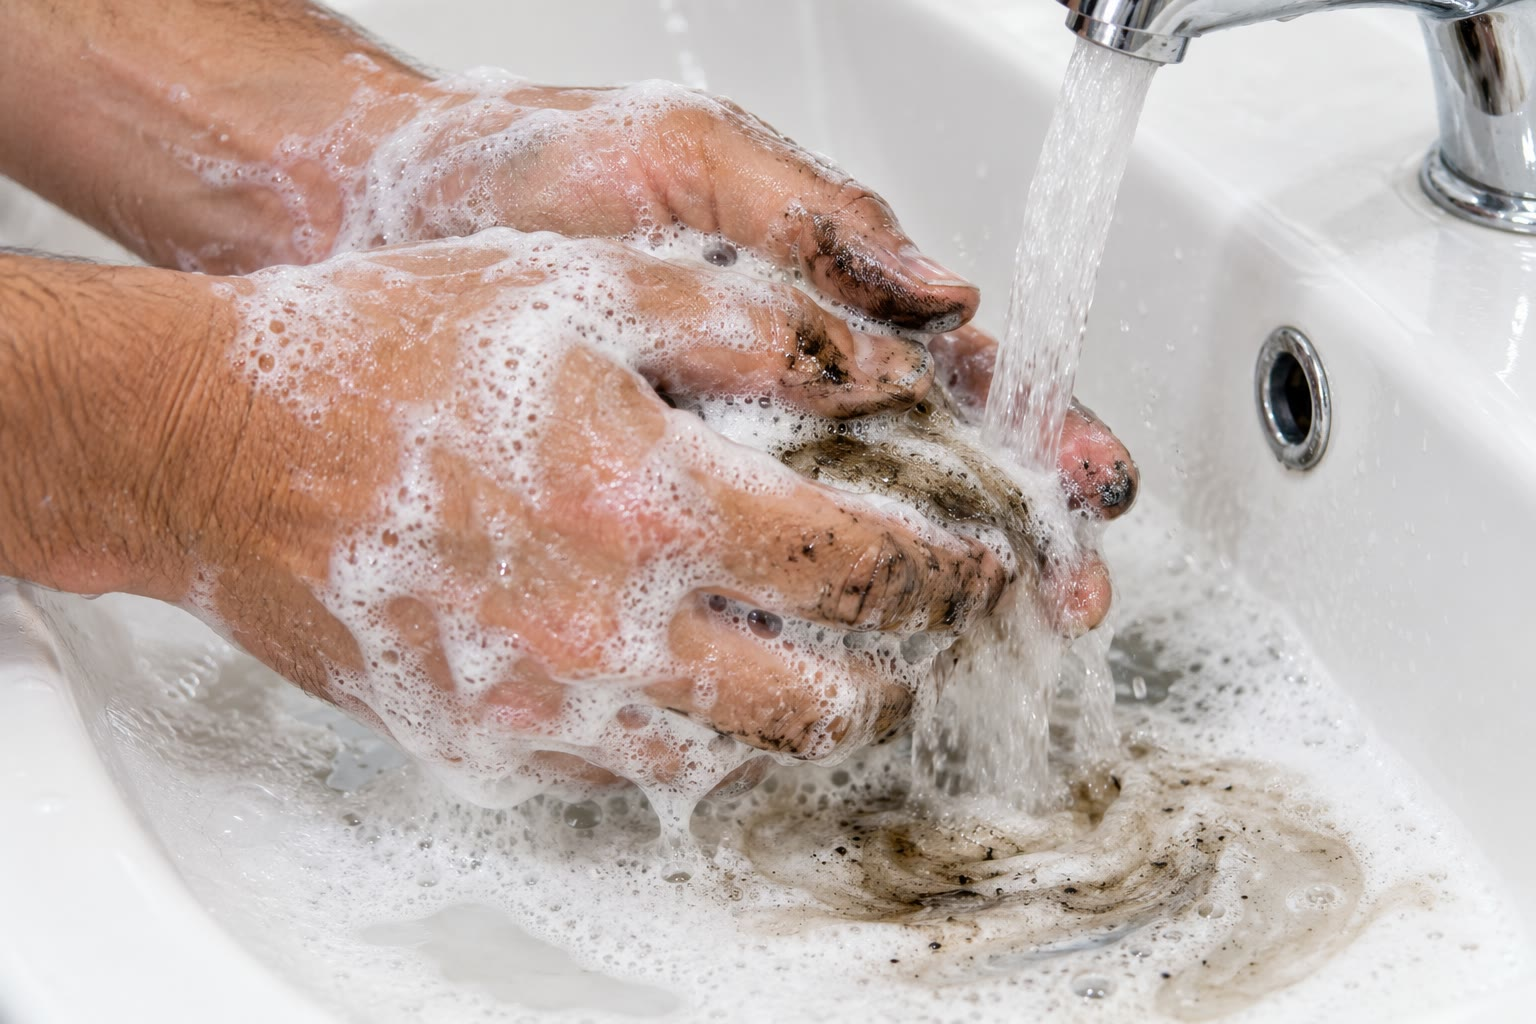
\includegraphics[width=0.48\linewidth]{images/book1/ai/g11-greasy-hands.jpg}

{\small Lavar mãos engorduradas: o sabão leva a gordura embora em
\omterm{def:g11:dissolution:amphiphilic}{micelas}.}
\end{omfigure}

\begin{remark}[Água dura e borra de sabão]\label{rem:g11:dissolution:scum}
A água dura contém muitos \omterm{def:g9:ions:ion}{íons} cálcio \ce{Ca^{2+}} e \omterm{def:g9:ions:ion}{íons} magnésio
\ce{Mg^{2+}}, dissolvidos das rochas por onde ela passou. Com os \omterm{def:g9:ions:ion}{íons}
estearato, eles formam um \omterm{def:g9:ions:precipitate}{precipitado} (\cref{ch:g9:ions}), o estearato de
cálcio:
\[
  \ce{2C17H35COO- + Ca^{2+} -> Ca(C17H35COO)2(s)} .
\]
Esse sólido acinzentado é a borra que forma um anel na pia, e cada \omterm{def:g9:ions:ion}{íon}
de sabão preso nela fica perdido para a lavagem: na água dura, o sabão
faz pouca espuma até que se tenha acrescentado o bastante para
precipitar todo o cálcio.
\end{remark}

\begin{omfigure}
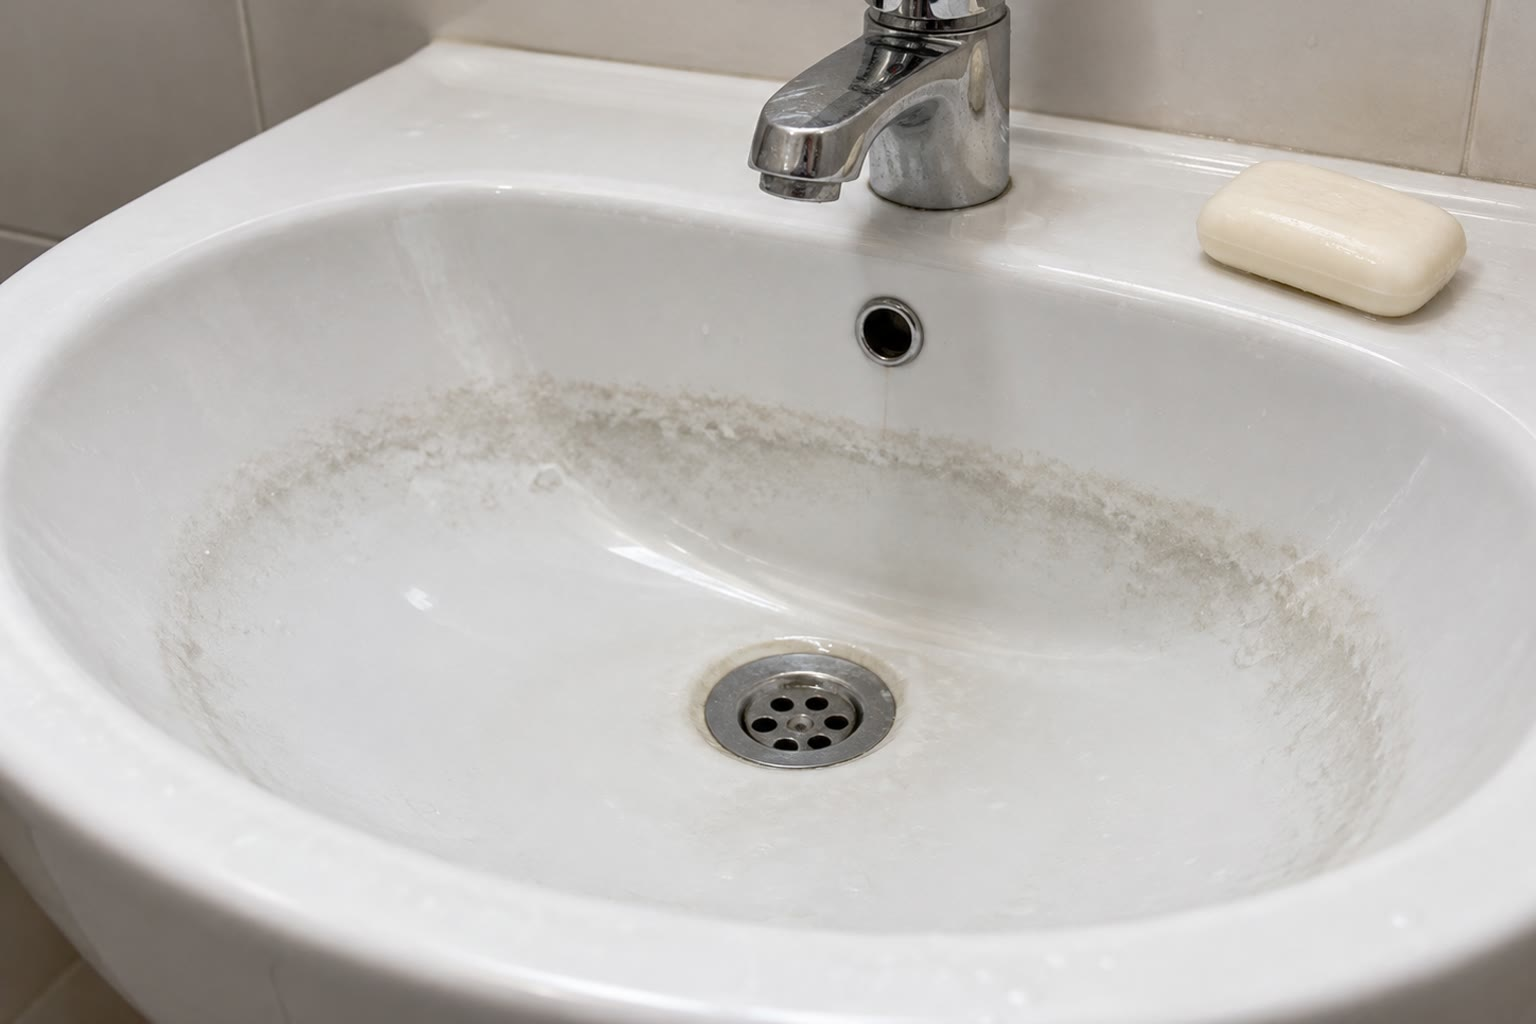
\includegraphics[width=0.45\linewidth]{images/book1/ai/g11-soap-scum.jpg}

{\small Borra de sabão numa pia: estearato de cálcio, \omterm{def:g9:ions:precipitate}{precipitado} pela
água dura.}
\end{omfigure}

\section{Exercícios}


\begin{exercise}[$\star$]\label{exo:g11:dissolution:1}
Escreva as equações de dissolução na água do cloreto de sódio \ce{NaCl},
do cloreto de cálcio \ce{CaCl2}, do sulfato de sódio \ce{Na2SO4} e do
cloreto de alumínio \ce{AlCl3}.
\end{exercise}

\begin{exercise}[$\star$]\label{exo:g11:dissolution:2}
Uma solução de sulfato de sódio tem $c = \qty{0.050}{mol/L}$. Dê as
concentrações dos \omterm{def:g9:ions:ion}{íons} sódio e dos \omterm{def:g9:ions:ion}{íons} sulfato.
\end{exercise}

\begin{exercise}[$\star$]\label{exo:g11:dissolution:3}
O que se entende por \omterm{def:g11:dissolution:solvation}{hidratação} de um \omterm{def:g9:ions:ion}{íon}? Que extremidade de uma
\omterm{def:g7:atoms-and-molecules:molecule}{molécula} de água aponta para um \omterm{def:g9:ions:ion}{cátion}, e qual aponta para um \omterm{def:g9:ions:ion}{ânion}?
Por quê?
\end{exercise}

\begin{exercise}[$\star$]\label{exo:g11:dissolution:4}
Dissolvem-se \qty{2.67}{g} de cloreto de alumínio para fazer
\qty{200.0}{mL} de solução. Calcule a concentração da solução e a de
cada \omterm{def:g9:ions:ion}{íon}.
\end{exercise}

\begin{exercise}[$\star$]\label{exo:g11:dissolution:5}
Identifique cada parte do \omterm{def:g9:ions:ion}{íon} estearato como \omterm{def:g11:dissolution:hydrophilic}{hidrofílica} ou \omterm{def:g11:dissolution:hydrophilic}{hidrofóbica},
e diga por quê.
\end{exercise}

\begin{exercise}[$\star\star$]\label{exo:g11:dissolution:6}
Que \omterm{def:g6:solutions-and-solubility:solute}{solvente}, água ou ciclo-hexano, você escolheria para \omterm{def:g2:mixing-and-dissolving:dissolve}{dissolver}: o
sal; a cera de vela (longas cadeias de hidrocarbonetos); o açúcar
(muitos grupos \ce{O-H}); o iodo? Justifique cada escolha.
\end{exercise}

\begin{exercise}[$\star\star$]\label{exo:g11:dissolution:7}
O etanol \ce{CH3-CH2-OH} se mistura com a água em todas as proporções,
mas o hexano \ce{C6H14} não se mistura com a água. Explique.
\end{exercise}

\begin{exercise}[$\star\star$]\label{exo:g11:dissolution:8}
Olhe a figura da \omterm{def:g11:dissolution:amphiphilic}{micela}. Por que as caudas ficam dentro e as cabeças
fora? Por que duas \omterm{def:g11:dissolution:amphiphilic}{micelas} não se juntam numa gota maior de gordura?
\end{exercise}

\begin{exercise}[$\star\star$]\label{exo:g11:dissolution:9}
Um aroma vegetal está dissolvido na água. Para extraí-lo, um químico pode
usar etanol ou ciclo-hexano. Qual deles é adequado, e por que o outro não
é (pense na miscibilidade)?
\end{exercise}

\begin{exercise}[$\star\star$]\label{exo:g11:dissolution:10}
Na \omterm{def:g10:chemical-species:extraction}{extração} do iodo, por que a camada de ciclo-hexano fica em cima? Que
camada é escoada pela torneira? Onde está o iodo no fim?
\end{exercise}

\begin{exercise}[$\star\star$]\label{exo:g11:dissolution:11}
Uma solução azul de sulfato de cobre é agitada com ciclo-hexano. O que
acontece com a cor azul? Explique.
\end{exercise}

\begin{exercise}[$\star\star\star$]\label{exo:g11:dissolution:12}
Que massa de cloreto de cálcio deve ser dissolvida para fazer
\qty{250.0}{mL} de uma solução em que $[\ce{Cl-}] = \qty{0.300}{mol/L}$?
\end{exercise}

\begin{exercise}[$\star\star\star$]\label{exo:g11:dissolution:13}
Verifica-se que uma amostra de água do mar contém \qty{0.010}{mol/L} de
\omterm{def:g9:ions:ion}{íons} cálcio e \qty{0.053}{mol/L} de \omterm{def:g9:ions:ion}{íons} magnésio. Explique por que o
sabão comum faz muito pouca espuma na água do mar. Quanto estearato de
sódio seria \omterm{def:g9:ions:precipitate}{precipitado} só pelos \omterm{def:g9:ions:ion}{íons} cálcio de um litro de água do mar?
\end{exercise}

\begin{exercise}[$\star\star\star$]\label{exo:g11:dissolution:14}
\qty{100.0}{mL} de solução de cloreto de sódio a \qty{0.20}{mol/L} são
\omterm{def:g2:mixing-and-dissolving:mix}{misturados} com \qty{100.0}{mL} de solução de cloreto de cálcio a
\qty{0.10}{mol/L}. Não se forma nenhum \omterm{def:g9:ions:precipitate}{precipitado}. Calcule as
concentrações de \ce{Na+}, \ce{Ca^{2+}} e \ce{Cl-} na \omterm{def:g6:pure-substances-and-mixtures:mixture}{mistura}, e
verifique que ela é neutra.
\end{exercise}

\begin{exercise}[$\star\star\star$]\label{exo:g11:dissolution:15}
% ledger: sol:I2-water, sol:I2-heptane, rho:heptane
O iodo \omterm{def:g2:mixing-and-dissolving:dissolve}{se dissolve} até cerca de \qty{0.3}{g} por litro de água e
\qty{17}{g} por quilograma de heptano. O heptano tem uma densidade de
cerca de \qty{0.68}{kg/L}. Quantas vezes mais iodo um litro de heptano
consegue conter que um litro de água? O que isso significa para uma
\omterm{def:g10:chemical-species:extraction}{extração}?
\end{exercise}

\section{Problema: o sabão e a água dura}

\begin{problem}[{Problema de fim de semana --- quanto sabão um banho de
água dura desperdiça em borra?}]
\label{pb:g11:dissolution:1}
% ledger: aw:Ca, aw:Mg, aw:C, aw:H, aw:O, aw:Na
Uma água da torneira contém \qty{120}{mg} de \omterm{def:g9:ions:ion}{íons} cálcio e \qty{24}{mg}
de \omterm{def:g9:ions:ion}{íons} magnésio por litro. Uma banheira é enchida com \qty{150}{L}
dela, e a pessoa que toma banho usa um sabão feito de estearato de
sódio, \ce{C17H35COONa}.

\medskip
\noindent\textbf{Parte I --- O que há na água.}
\begin{enumerate}
  \item De onde vêm os \omterm{def:g9:ions:ion}{íons} cálcio e magnésio da água da torneira?
  \item Calcule as \omterm{def:g10:concentration-and-dilution:molar-concentration}{concentrações molares} dos \omterm{def:g9:ions:ion}{íons} cálcio e dos \omterm{def:g9:ions:ion}{íons}
        magnésio.
  \item Os \omterm{def:g9:ions:ion}{íons} cálcio vêm acompanhados de \omterm{def:g9:ions:ion}{íons} hidrogenocarbonato,
        \ce{HCO3-}, como se tivesse sido dissolvido hidrogenocarbonato
        de cálcio \ce{Ca(HCO3)2}. Escreva essa equação de dissolução, e
        deduza a concentração de \omterm{def:g9:ions:ion}{íons} hidrogenocarbonato que acompanha o
        cálcio.
  \item Que quantidade de \omterm{def:g9:ions:ion}{íons} cálcio a banheira contém?
\end{enumerate}

\medskip
\noindent\textbf{Parte II --- O sabão.}
\begin{enumerate}[resume]
  \item Calcule a \omterm{def:g10:the-mole:molar-mass}{massa molar} do estearato de sódio.
  \item Escreva a sua equação de dissolução na água.
  \item Que parte do \omterm{def:g9:ions:ion}{íon} estearato é \omterm{def:g11:dissolution:hydrophilic}{hidrofílica}, e qual é \omterm{def:g11:dissolution:hydrophilic}{hidrofóbica}?
        Por que ele é chamado de \omterm{def:g11:dissolution:amphiphilic}{anfifílico}?
  \item Descreva uma \omterm{def:g11:dissolution:amphiphilic}{micela}, e explique como ela remove a gordura da
        pele.
  \item Por que o sabão deve ser dissolvido na água, e não no óleo, para
        lavar?
\end{enumerate}

\medskip
\noindent\textbf{Parte III --- A borra.}
\begin{enumerate}[resume]
  \item Escreva a equação da \omterm{def:g9:ions:precipitate}{precipitação} do estearato de cálcio.
        Verifique que ela está balanceada em carga.
  \item Preencha a \omterm{def:g10:reaction-progress-table:extent}{tabela de avanço} para \qty{1.00}{L} da água da
        torneira e um excesso de \omterm{def:g9:ions:ion}{íons} estearato. Que \omterm{def:g7:chemical-reactions:reactant}{reagente} é
        limitante?
  \item Que quantidade de \omterm{def:g9:ions:ion}{íons} estearato é perdida por litro para o
        cálcio?
  \item Calcule a \omterm{def:g10:the-mole:molar-mass}{massa molar} do estearato de cálcio, e a massa de borra
        formada por litro.
  \item O estearato de magnésio precipita do mesmo modo. Que quantidade
        de estearato os \omterm{def:g9:ions:ion}{íons} magnésio tomam por litro?
\end{enumerate}

\medskip
\noindent\textbf{Parte IV --- O banho.}
\begin{enumerate}[resume]
  \item Que quantidade de \omterm{def:g9:ions:ion}{íons} estearato o cálcio da banheira inteira
        precipita?
  \item Que massa de sabão é essa?
  \item Somando o magnésio, que massa de sabão é desperdiçada ao todo?
  \item As barras de sabão pesam cerca de \qty{100}{g}. Quantas barras
        o cálcio sozinho consome?
  \item Dê a resposta final: que massa de sabão o cálcio de um banho de
        \qty{150}{L} dessa água desperdiça em borra?
\end{enumerate}
\end{problem}